

\chapter{Power Spectral Density}

\section{Introduction}

Spectral Analysis: characterize power distribution over frequency using finite amount of time series data (chapter 1 in \cite{book_Spectral_Analysis_Stoica}).\\

The PSD concept is important to use in communication signals, where they are random in nature, and hence they have infinite power. To analyze such signals, PSD concept is used (see section 1.2.4 \cite{books_digital_comm_fundamentals_Sklar})

For a nice introduction and reviewing concept:\\

\begin{itemize}
    \item See chapter 1 (mainly 1.3) in \cite{book_Spectral_Analysis_Stoica}

\end{itemize}

\section{Pwelsh Method}

We start by simple simulation of a sin function:

\begin{equation}
    x(t) \, = \, A \, \sin{2 \pi f \, t} \quad \text{where } f \, = \, 500 \text{Hz and } A \, = \, \sqrt{2}
\end{equation}

We take $F_s \, = \, 4$KHz and number of point to generate 1024.\\

Analytically, power of $x(t) \, = \, \displaystyle\frac{A^2}{2} \, = 1$ Watt $\rightarrow 10 \log_{10} (\, 1\, ) \, = \, 0$ dBW/Hz.

\subsection{Reminder of Power Notion}

See section 2.5 in \cite{books_principle_of_system_Ziemer}.

\begin{itemize}
    \item PSD gives power per frequency components $\leftrightarrow$ Watt/Hz
    
    \item The \tbi{total power} or \tbi{average power} is the sum of the PSD (integration to be precise)
    
    \item For sin and cos signals:
    
    \begin{itemize}
        \item PSD is $\displaystyle\frac{A^2}{4}$
        
        \item Average power $= \displaystyle\frac{A^2}{4} \, + \, \displaystyle\frac{A^2}{4} \, = \, \displaystyle\frac{A^2}{2}$
    \end{itemize}
    
\end{itemize}

\subsection{Matlab Simulation}

In Maltab, we can use the \verb|pwelsh| function to compute the average power where:

\verb|[pxx,f]= pwelch(signal,window,n_overlapp,nfft,fs);| where:

\begin{itemize}

    \item \verb|nfft = Nb_samples = | 1024
    
    \item \verb|window = rectwin(nfft);|
\end{itemize}

\autoref{fig:PSD_Com:Demo_PSD_Sin} show the results of the simulation.

\begin{figure}[h]
\centering
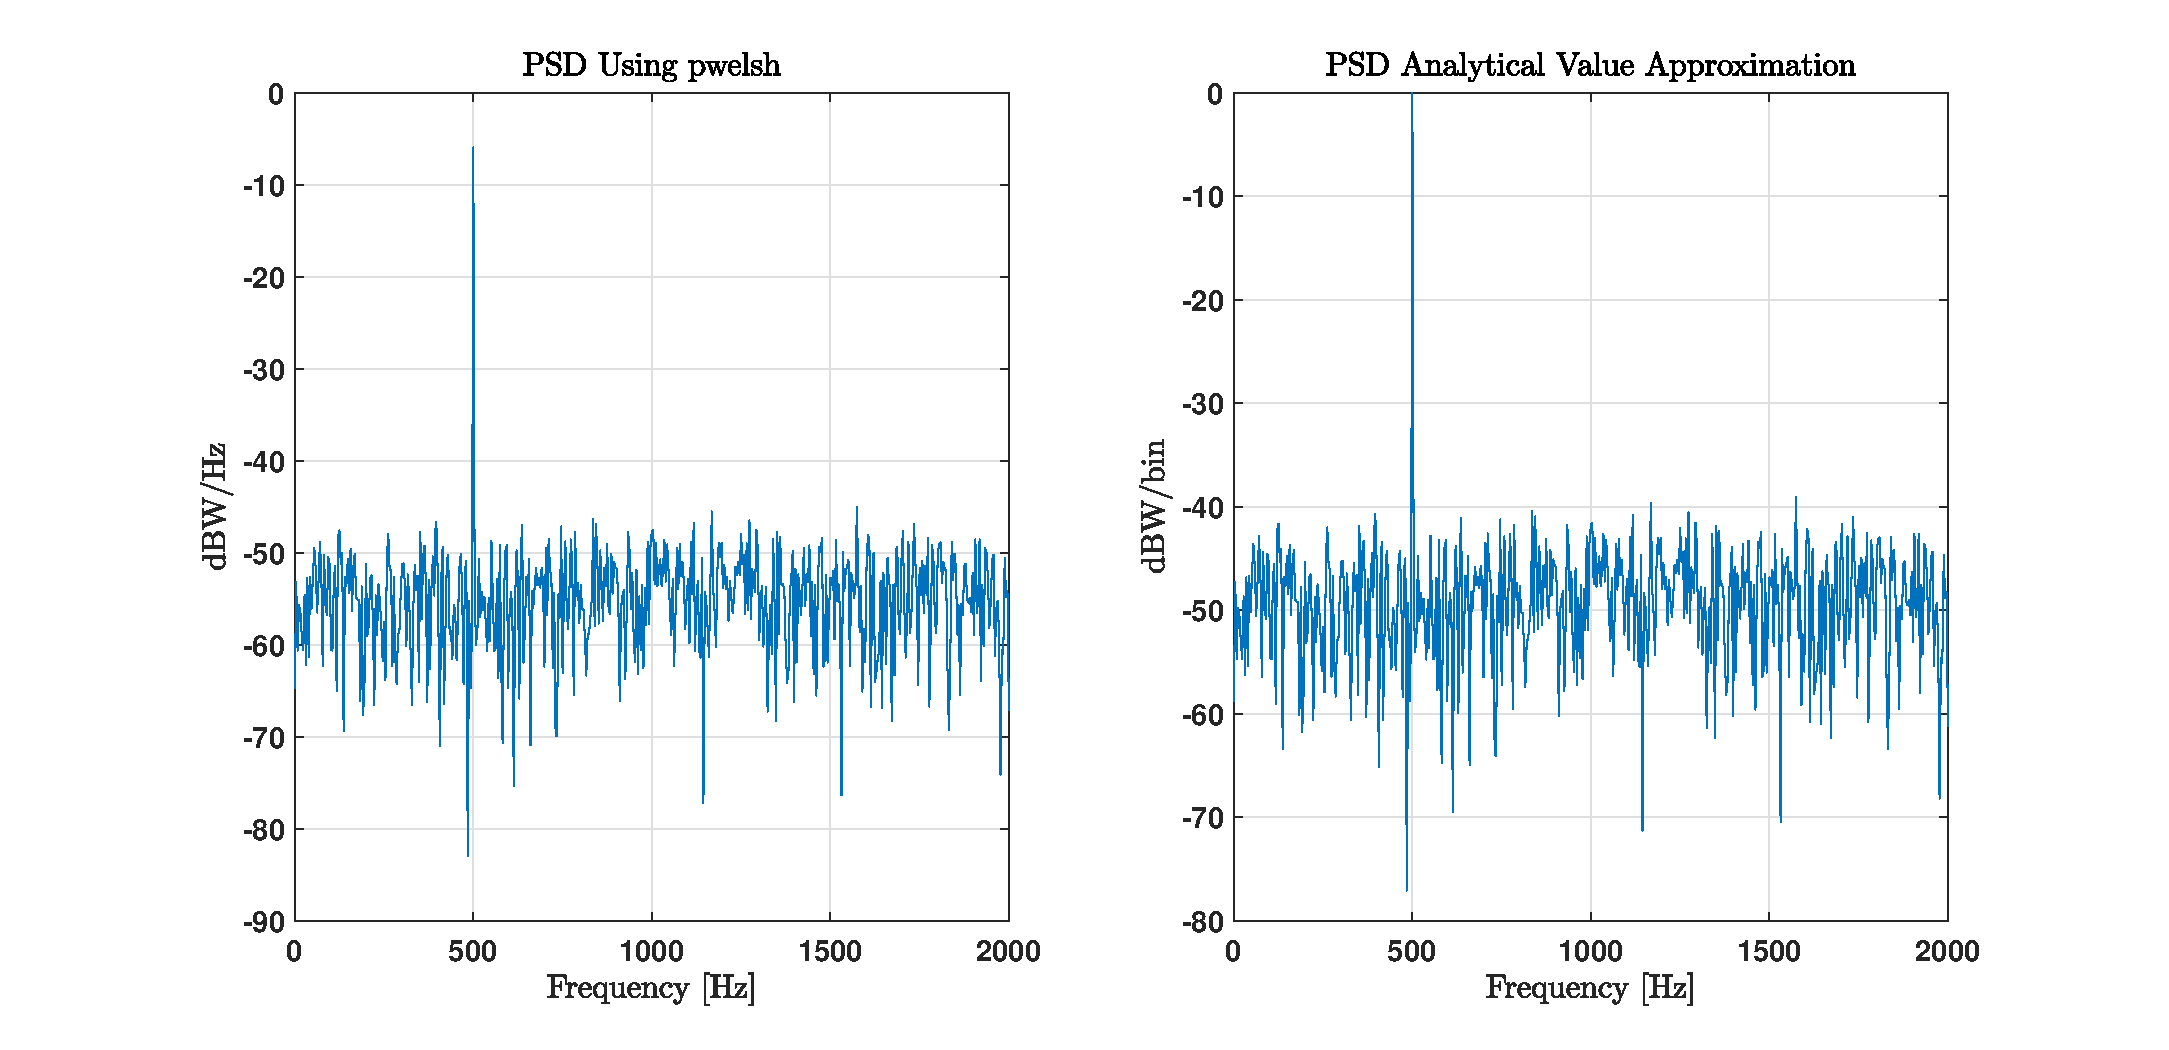
\includegraphics[scale=0.5]{Figures/PSD_Com/Demo_PSD_Sin}
\caption{Sin Demo using pwelsh function}
\label{fig:PSD_Com:Demo_PSD_Sin}
\end{figure}

The result of the \verb|pwelsh|, which is \verb|10log10(pxx)|, give a value of $\approx$ -5.9 dBW, which is different from 0 dBW.\\

So how to move from -5.9 dBW $\rightarrow$ 0 dBW ?

What we need to do is to multiply the value of \verb|pxx|, which is W/Hz, and convert to Watt/bin, and this done as:

\begin{equation}
 \text{Pbin (W/bin) = pxx (W/Hz) * Fs/nfft (Hz/bin)}
\end{equation}

\subsection{Windowing,Overlapping}

\todo{PSD:Windowing,Overlapping}.

\newpage
\section{Equivalent noise bandwidth(ENBW)}

\begin{itemize}

\item \underline{source:} \url{https://analog.intgckts.com/equivalent-noise-bandwidth/}.

Contains nice definition, and graphics

\item  MATLAB source for simulation: \url{https://fr.mathworks.com/help/signal/ref/enbw.html#btrihsq-1}

\end{itemize}

\todo{ENBW} \underline{\textit{ENBW}:} \textit{To redo a proper documentation and simulation from the resources above}. 